% !TEX root = 99_main.tex

The experiment, consisting of 15 users each equipped with a fitbit over a month, produced a dataset of [INSERT NUMBER HERE] data points. Each data point is effectively a survey of the user at a particular time. The results presented in this section is a demonstration of the type of analysis that can be conducted using data acquired from the cozie watch-face.

\subsection{Evaluational of user comfort over a day}

Figure \ref{fig:hourPlot} details a simple heat-map where the user comfort feedback is mapped to the hour of the day. Users appear to be comfortable on average [INSERT NUMEBR HERE] \% of the time, and there are no statistically significant trends during working hours (9:00 - 17:00). Variations in user comfort feedback during the day can be used to infer an issue within the building.

It is interesting to note that there is on average [INSERT NUMBER HERE] times more responses in the hours of 9:00, 11:00, 13:00, 15:00, and 17:00 when the occupant is buzzed and forced to give feedback. Nevertheless there are still significant amounts of responses made outside these times through the motivation of the participants themselves. Figure \ref{fig:responseRate} details the daily responses from the participants, and no observable decrease in responses can be made. Dips in responses naturally occur during the weekend. 


\begin{figure}
\centering
	\begin{subfigure}[t]{0.5\textwidth}
	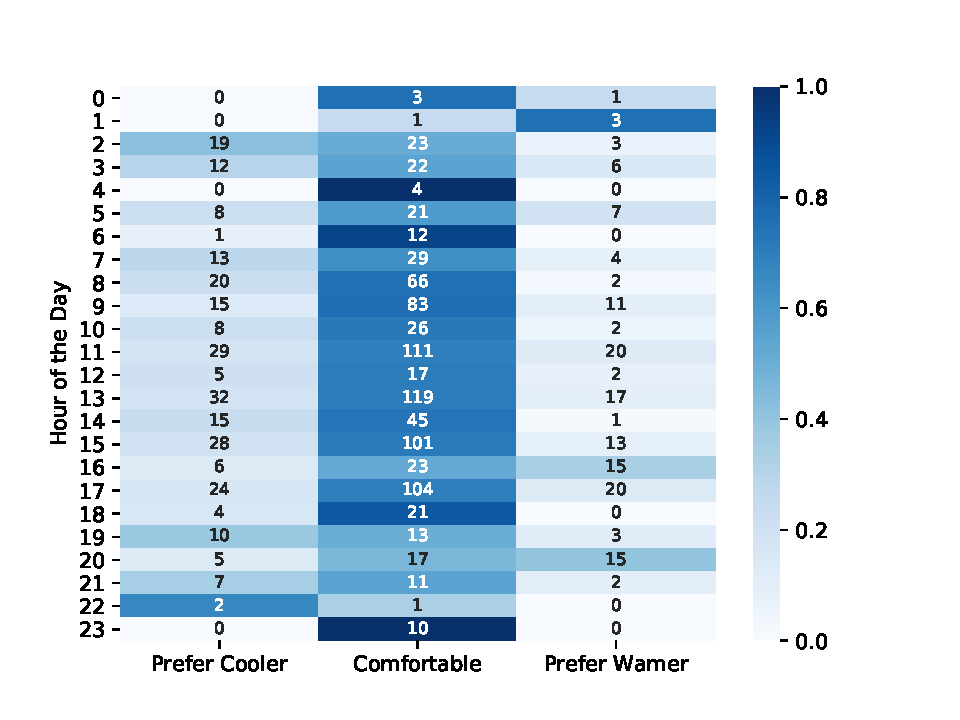
\includegraphics[width=\textwidth, trim= 0cm 0cm 0cm 0cm,clip]{hourPlot.pdf}
	\caption{(a)}
	\label{fig:hourPlot}
	\end{subfigure}
	\begin{subfigure}[t]{0.49\textwidth}
	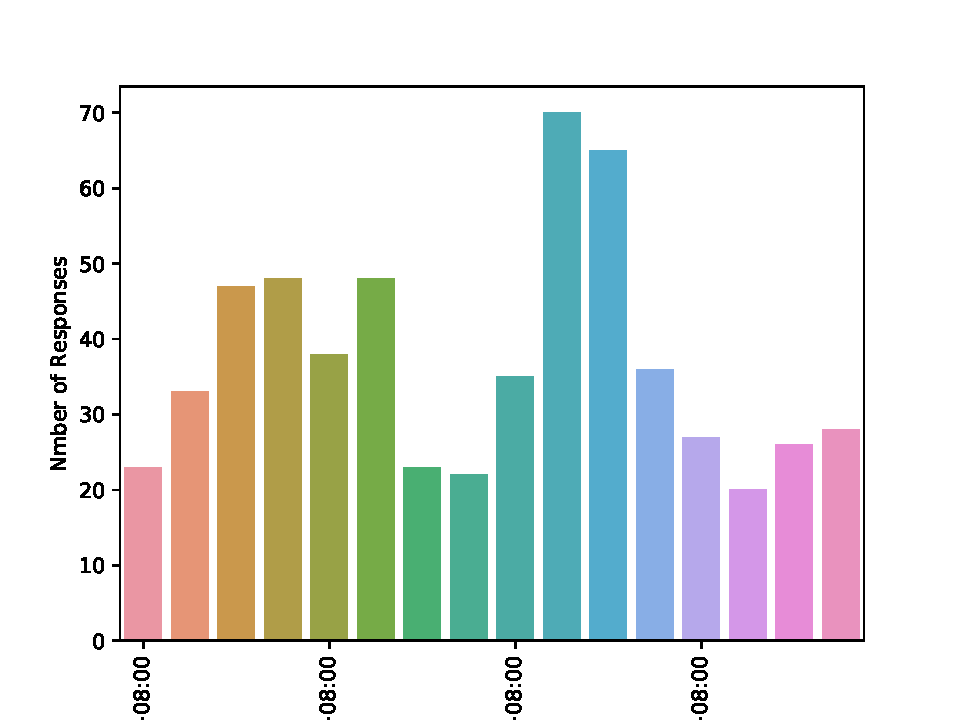
\includegraphics[width=\textwidth, trim= 0cm 0cm 0cm 0cm,clip]{response_rate.pdf}
	\caption{(b)}
	\label{fig:responseRate}
	\end{subfigure}
	\caption{(a) Aggregation of user feedback mapped to the hour of the day that feedback was given. Annotations within the heat-map detail the absolute response value, while the colour gradient relates to the normalised values (b) Daily responses during the course of the evaluation period. The dips in the graph are weekends}
\end{figure}


\begin{figure}
    \centering
    \begin{subfigure}[t]{0.3\textwidth}
        \centering
        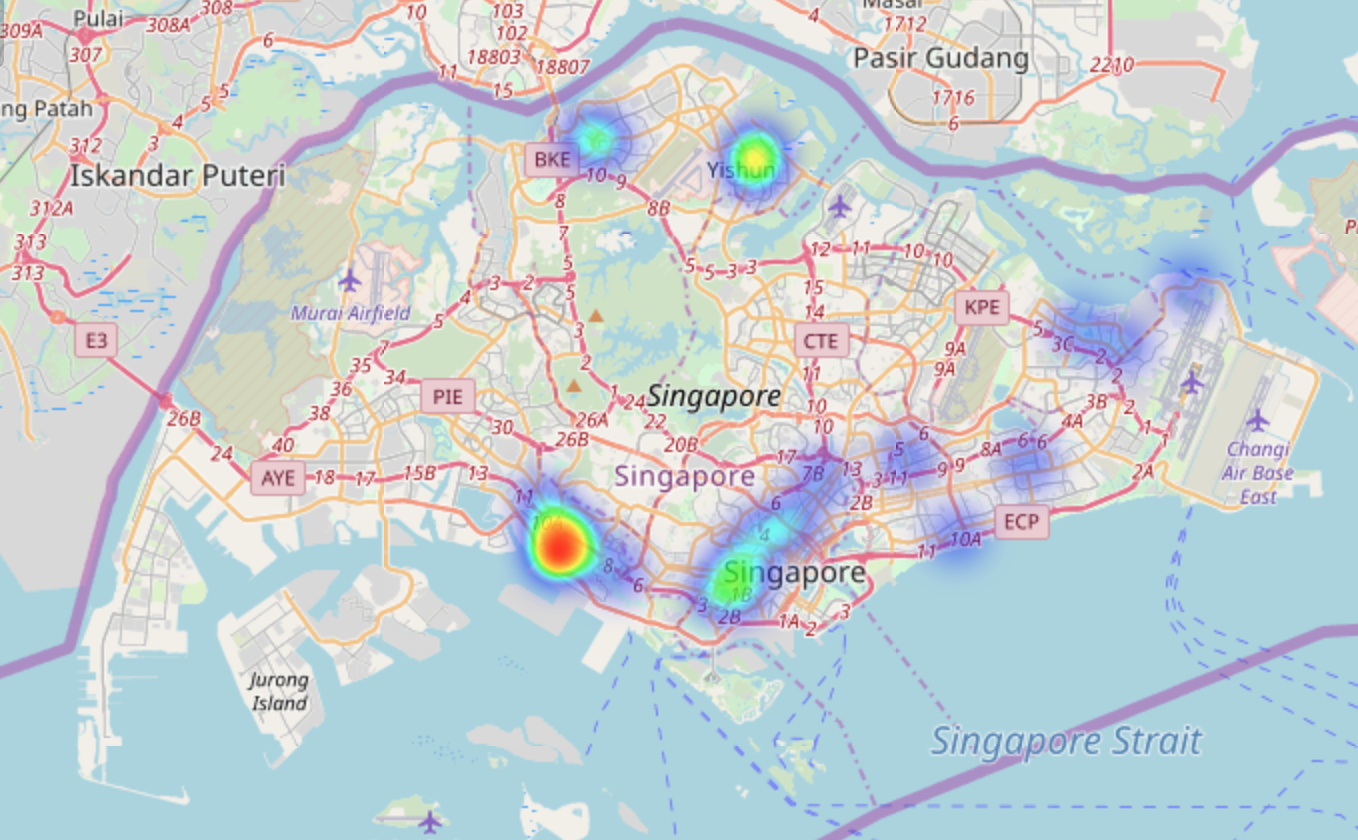
\includegraphics[height= 3cm]{map_singapore.png}
        \caption{(a)}
    \end{subfigure}
    \begin{subfigure}[t]{0.3\textwidth}
        \centering
        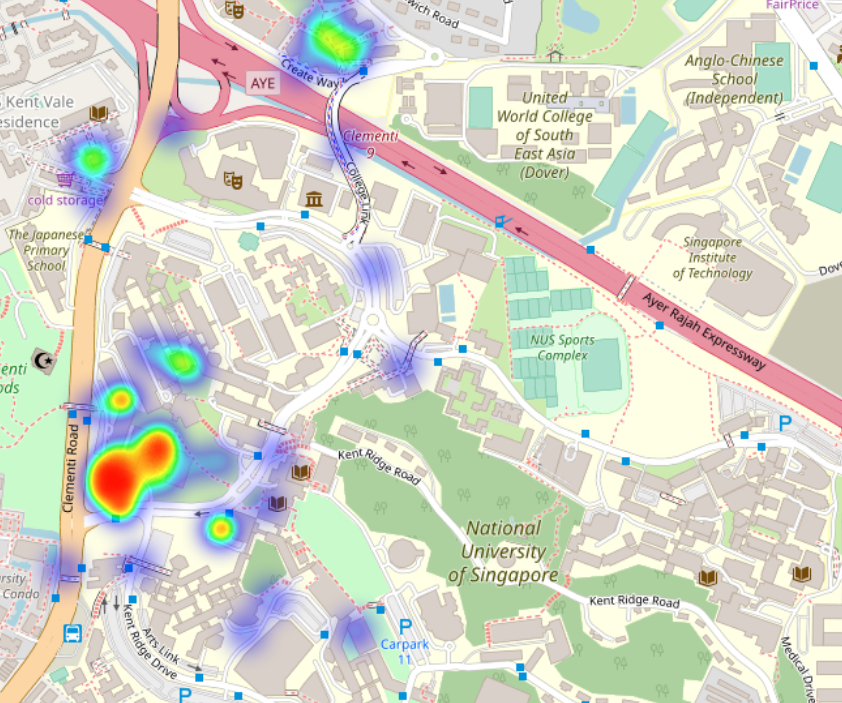
\includegraphics[height= 3cm]{map_nus.png}
        \caption{(b)}
    \end{subfigure}
    \begin{subfigure}[t]{0.3\textwidth}
        \centering
        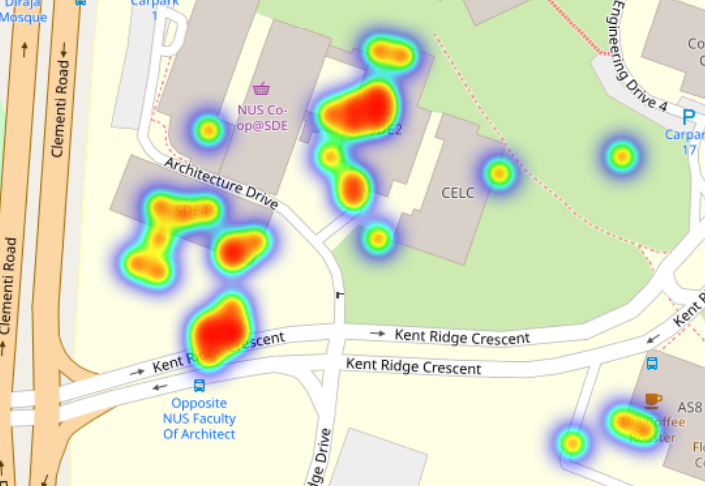
\includegraphics[height= 3cm]{map_sde.png}
        \caption{(c)}
    \end{subfigure}
    \caption{Map of responses. From left to right, the city of Singapore, National University of Singapore, and the School of Design and Environment. The experiment was conducted at co-working spaces at the school of design and environment, however responses are seen throughout Singapore. Note that these results only show 172 of the [INSERT NUMBER] total responses as GPS localisation often failed indoors.}
    \label{fig:map}
\end{figure}


\subsection{Influence of Individual Users}
\label{ch:userResults}

Individual user feedback can be clustered using un-supervised learning techniques. In this example, we use a hierarchal k-means clustering based on euclidean distance using the Nearest-Point-Algorithm. The results, shown in Figure \ref{fig:clustering}, show four distinct clusters of users. 
%Users that are comfortable 100\% of the time, users that are comfortable 60-80 \% of the time, those that are comfortable 50\% of the time and generally would prefer it cooler, those that are comfortable 50\% of the time and would prefer it both warmer and cooler. 
Understanding and defining these differences in user preferences can be used to recommend spaces that may better suit the needs of the occupant. For example, User 5 and User 10 can be recommended working spaces that are on average cooler. User 13 on the other hand appears to have a broad comfort spectrum. 

It is importat to note that the data is not representative of a single space. As shown in Figure \ref{fig:map}, responses were made throughout Singapore. GPS data can support in localising responses to individual buildings, but also comes with issues which will be discussed in Section \ref{ch:localisation}.


%It is important to note here that the data is not entirely representative of a single building space, as the user may have given feedback while having lunch outside. There are even feedback results made outside of working hours as seen in \ref{fig:hourPlot} \ref{fig:responseRate}. Conclusions such as "Building Zone A was comfortable 80\% of the time" can therefore not be made. This will be further discussed in Section \ref{ch:discussion}.


\begin{figure}
    \begin{subfigure}[t]{0.49\textwidth}  
    \centering
        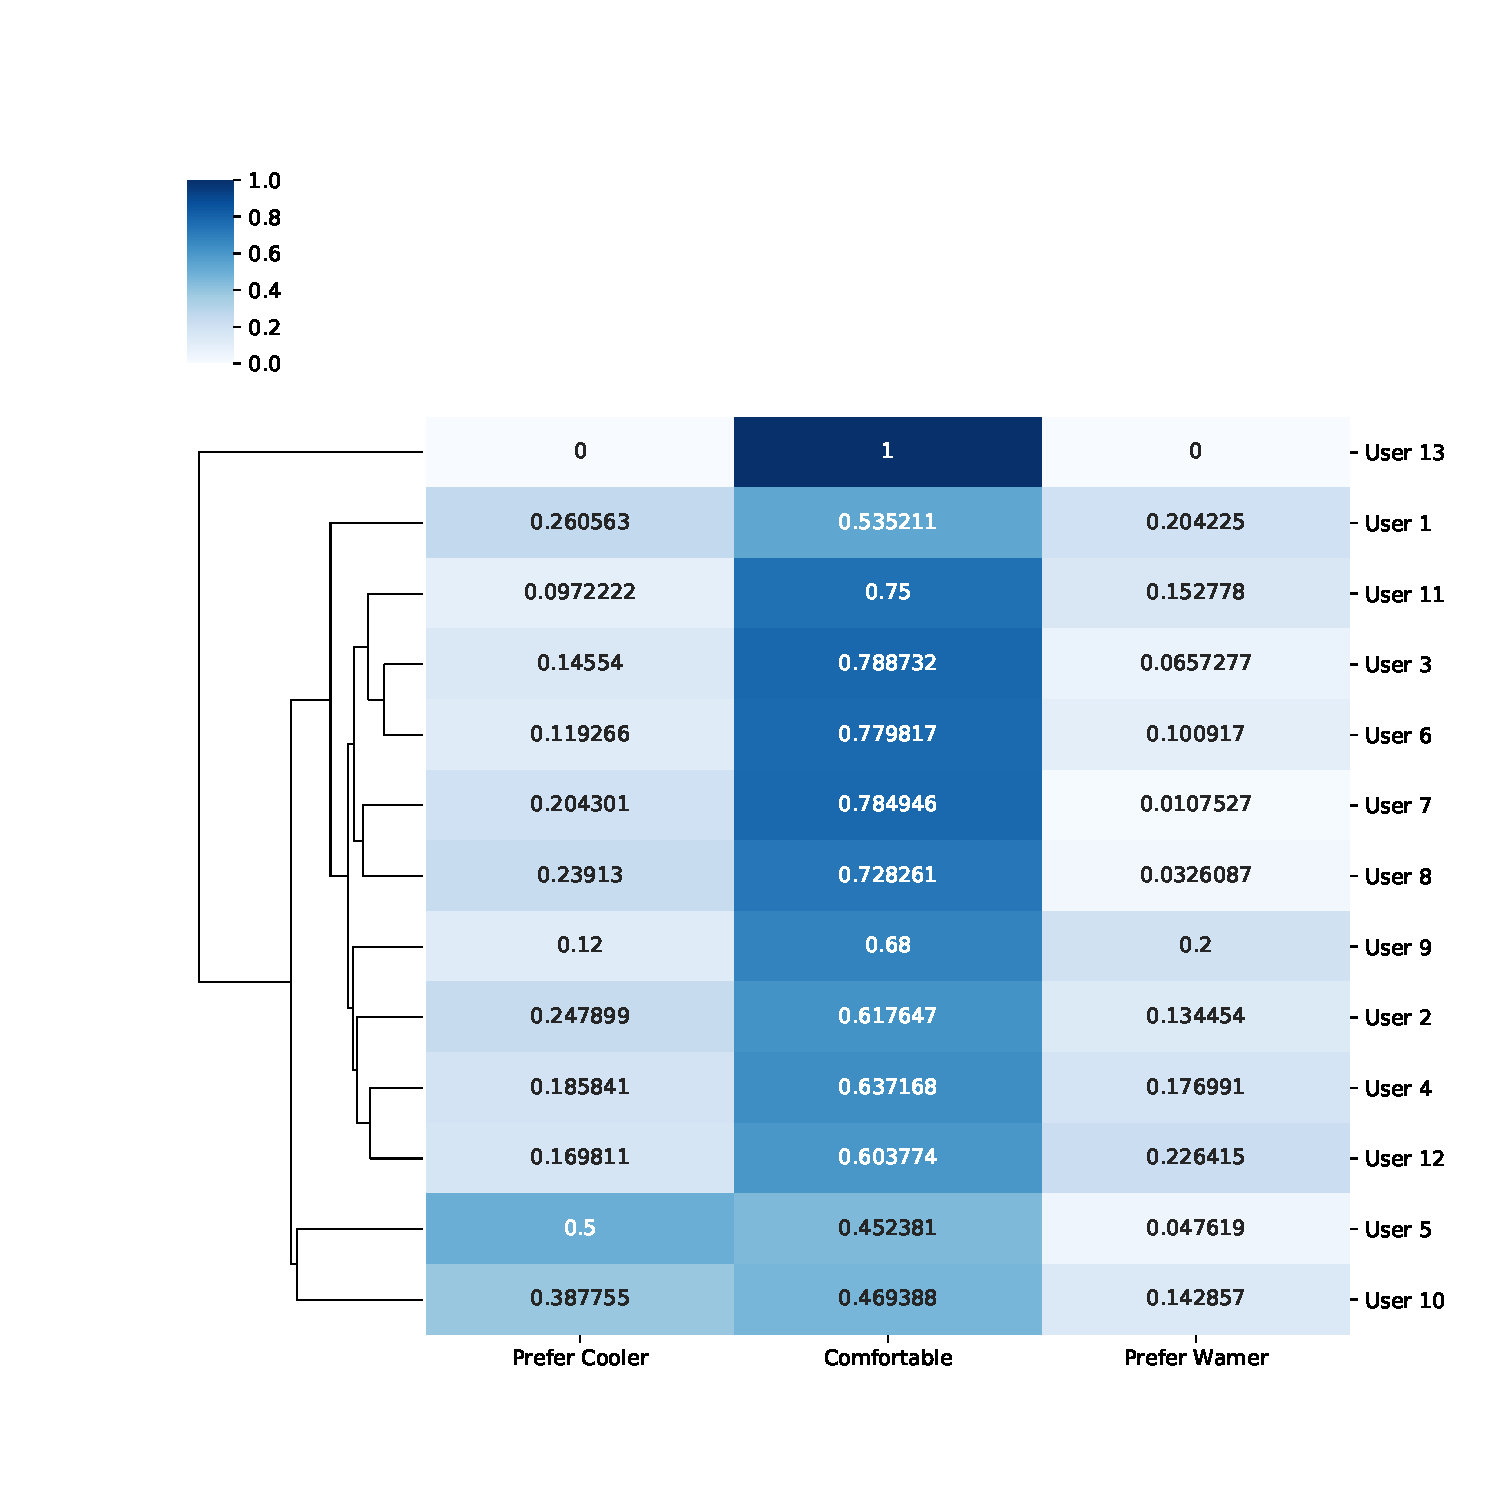
\includegraphics[width=\textwidth, trim= 0cm 0cm 0cm 0cm,clip]{cozie_users.pdf}
		\caption{(a)}
		\label{fig:userPlot}
    \end{subfigure}
    \begin{subfigure}[t]{0.49\textwidth}
    \centering
        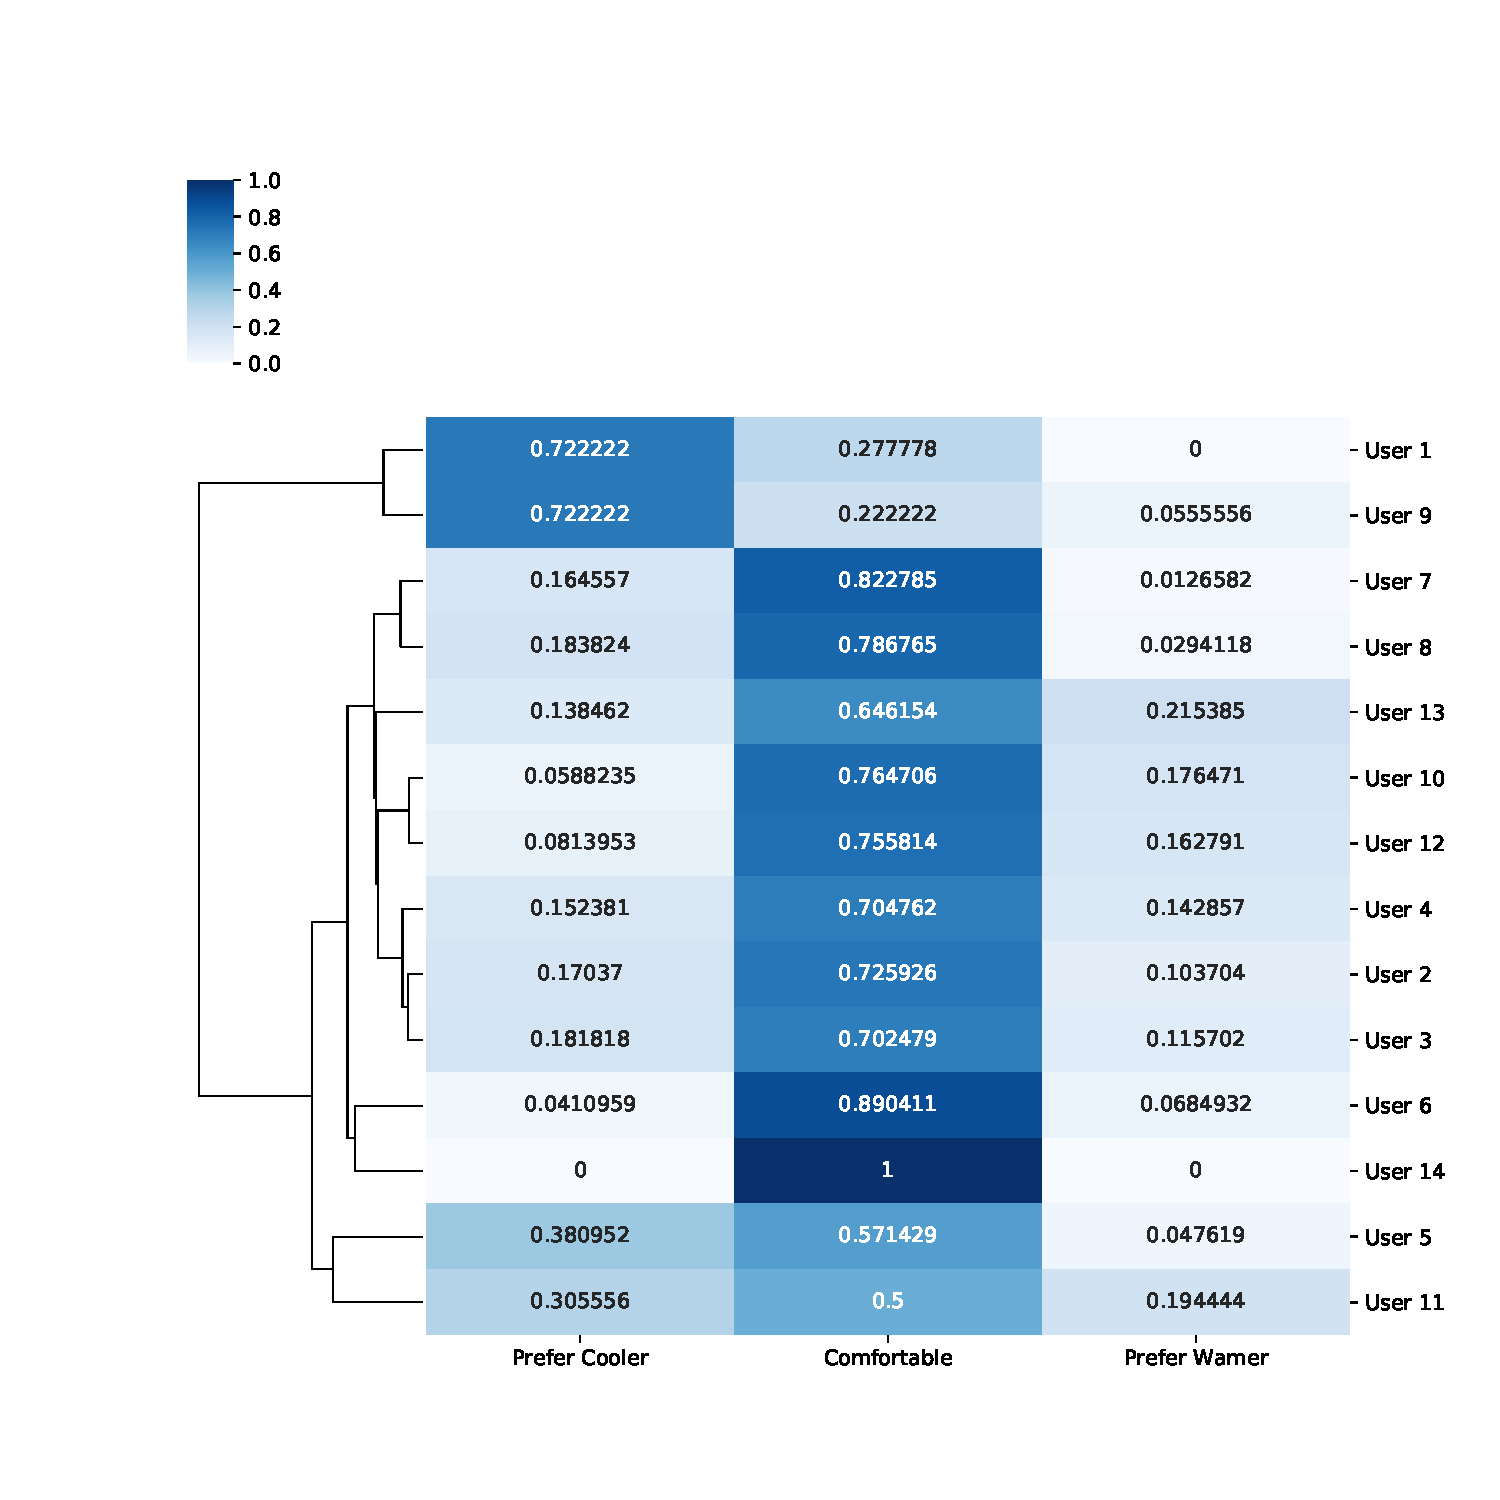
\includegraphics[width=\textwidth, trim= 0cm 0cm 0cm 0cm,clip]{cozie_users_lowheart.pdf}
		\caption{(b)}
		\label{fig:lowHeartUsers}
    \end{subfigure}
    \caption{Clustering of user feedback using hierarchal k-means. (a) The full results show four distinct clusters, (b) filter by heart rate that is less than 100 beats per minute}
    \label{fig:clustering}
\end{figure}




\subsection{Influence of Heart-Rate}

It is widely known that heart-rate influences metabolic activity, and therefore an occupants comfort preference. Figure \ref{fig:heartHist} details the number of responses for each thermal response based on the heart rate. [INSERT NUMBER HERE ] \% of "Prefer Cooler" responses occurred during higher metabolic activity when the heart rate was greater than 100 beats per minute. If we filter out these responses,and apply the same algorithms detailed in Section \ref{ch:userResults}, we see a slightly different response and clustering pattern, as shown in Figure \ref{fig:lowHeartUsers}. 



\begin{figure}
    \begin{subfigure}[t]{0.49\textwidth}  
    \centering
	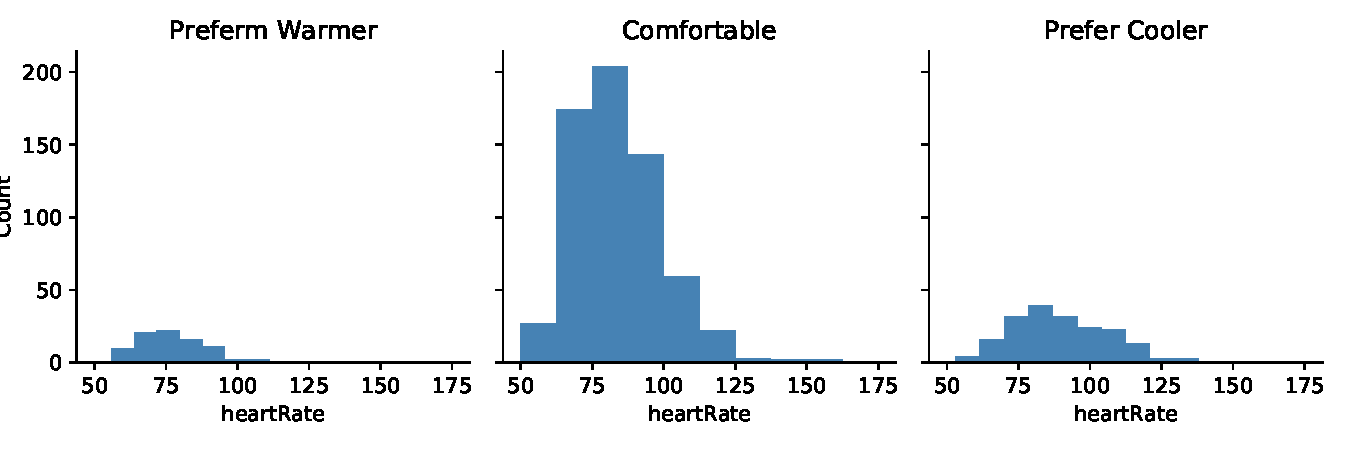
\includegraphics[width=\textwidth, trim= 0cm 0cm 0cm 0cm,clip]{heartHist.pdf}
	\caption{(a)}
	\label{fig:heartHist}
    \end{subfigure}
    \begin{subfigure}[t]{0.49\textwidth}
    \centering
		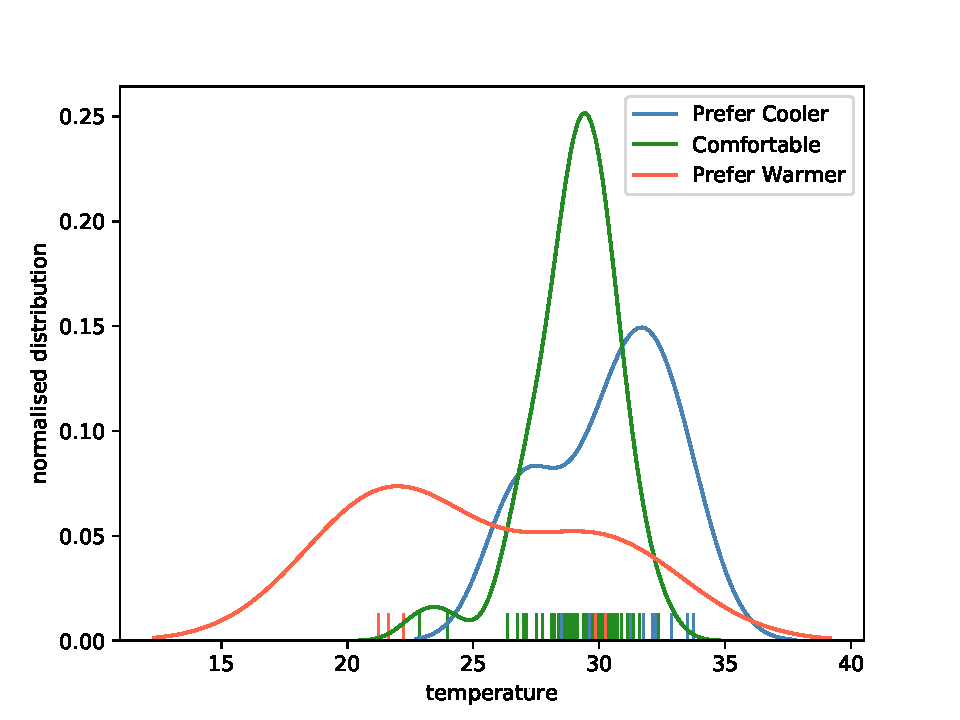
\includegraphics[width=\textwidth, trim= 0cm 0cm 0cm 0cm,clip]{temperatureHist.pdf}
		\caption{(b)}
		\label{fig:tempHist}	
    \end{subfigure}
    \caption{ Normalised distribution of the response type based on (a) heart rate (b) temperature. Note that the normalisation for "prefer warmer" is skewed due to the lack of responses of this type}
\end{figure}



\subsection{Combination with Sensor Data}

Combining the cozie watch face, with the "strap-pack", an environmental sensor addition to the watch face opens another dimension of analysis. User responses are mapped to the environmental condition at which they are exposed to, which can provide a high quality labeled data set for training data driven models. Figure \ref{fig:tempHist} detail the temperatures at which responses were mapped. Note that the temperature of the strap sensor is on average 0.8 $^\circ$C warmer than the surrounding environment due to the influence of body temperature. 


% convert time to bars
% one heart rate filter showing. Groups of similar behaving people. Group 1-4. What are the coincidental ranges of data belonging to these groups. 